%!TEX program=xelatex
\documentclass[utf8]{book}
\usepackage[heading,UTF8]{ctex}
\usepackage{titletoc}
\usepackage{titlesec}
\usepackage[a4paper,text={125mm,195mm},centering,left=1in,right=1in,top=1in,bottom=1in]{geometry}
\usepackage{imakeidx}
\usepackage{multicol}
\usepackage{hyperref}
\usepackage{amsmath, amssymb, amsfonts, mathrsfs}

\DeclareFontFamily{U}{mathx}{\hyphenchar\font45}
\DeclareFontShape{U}{mathx}{m}{n}{<-> mathx10}{}
\DeclareSymbolFont{mathx}{U}{mathx}{m}{n}
\DeclareMathAccent{\widebar}{0}{mathx}{"73}

\usepackage{graphicx}
\usepackage{subfig}
\usepackage{tikz,pgf}
\usepackage{color, xcolor}
\usepackage{pgfplots}
\pgfplotsset{compat=1.16}

%On Linux
%\setmainfont{DejaVu Sans}
\setCJKmainfont{Noto Serif CJK SC}
\setCJKsansfont{Note Sans CJK SC}
%On Windows 
%\setmainfont{Times New Roman}
%\setCJKmainfont{宋体}
%\setCJKsansfont{黑体}

\makeindex
\bibliographystyle{plain}



\begin{document}

\chapter{绪论}
\section{定义}
\section{课程内容}
\section{教学安排}


%\chapter{控制方程}
\section{纳维-斯托克斯方程}
\subsection{模型}
\subsection{连续性方程}
\subsection{运动方程}
\section{雷诺应力平均方程}
\subsection{紊流基础特征}
\subsection{紊流连续性方程}
\subsection{紊流运动方程}
\subsection{紊流模型}
\section{二维浅水方程}
\subsection{浅水假设}
\subsection{浅水连续性方程}
\subsection{浅水运动方程}
\subsection{浅水方程形式}
\section{一维圣维南方程}
\subsection{一维连续性方程}
\subsection{一维运动方程}
\subsection{圣维南方程形式}


\chapter{有限差分法}
上一章推导的控制方程的解析解,如果可以得出,将可以给出所有因变量在求解域上连续函
数。然而,除了个别极其简单的流动情况,这类方程的解析解往往很难获得。因此,我们只
能退而求其次,通过将连续的空间和时间分割成不连续的散点(分别称为网格点和时间节点
),并将控制方程在这些散点上离散,得出与原方程近似但可求解的代数方程组,最终得出
原方程在这些散点上的近似解。

在实际的数值模拟过程中,网格点或时间节点的划分是不均匀的。为了后续推导方便,本章
假定网格点和时间节点的间距都是均匀分布的。此外,本章只关注结构网格,对非结构网格
可参见其他参考书。

\section{泰勒展开}
考虑一个$x$的连续函数$f(x)$在$x$处的所有阶导数都存在。那么,$f$在点$x+\Delta x$
处的值可以通过在点$x$处的泰勒级数展开来估算。
\begin{equation}
  f(x+\Delta x)
  =
  f(x)
  +
  \frac{\partial f}{\partial x}\Delta x
  +
  \frac{\partial^{2} f}{\partial x^{2}}\frac{\Delta x^{2}}{2}
  +
  \cdots
  +
  \frac{\partial^{n} f}{\partial x^{n}}\frac{\Delta x^{n}}{n!}
  +
  \cdots
\end{equation}

假定$f(x)=\sin{2\pi x}$,且已知$x=0.2$处,函数值$f=0.9511$。我们希望估算
$x+\Delta x=0.22$处的函数值。根据方程表达式,该点的精确值为0.9823。首先,我们利
用泰勒级数展开的第一项来估算,有
\begin{equation}
  \begin{aligned}
    f(x+\Delta x) \approx f(x)  \\
    f(0.22) \approx f(0.2) = 0.9511
  \end{aligned} 
\end{equation}
估算值的相对误差为$(0.9823-0.9511)/0.9823=3.176\%$。接着,我们利用展开式的前两项
来估算,有
\begin{equation}
  \begin{aligned}
    f(x+\Delta x) &\approx f(x) + \frac{\partial f}{\partial x}\Delta x
  \\
    f(0.22) &\approx f(0.2) + 2\pi\cos{[2\pi(0.2)]}(0.02)
    \\
            &\approx 0.9511 + 0.388 = 0.9899
\end{aligned}
\end{equation}
估算值的相对误差为$(0.9899-0.9823)/0.9823=0.775\%$,相比于第一次的估算值更加接近
精确值。最后,为了获得更加精确的估算值,我们可以利用展开式的前三项,有
\begin{equation}
  \begin{aligned}
    f(x+\Delta x) &\approx f(x) + \frac{\partial f}{\partial x}\Delta x
    +
    \frac{\partial^{2} f}{\partial x^{2}}\frac{(\Delta x)^{2}}{2}
  \\
    f(0.22) &\approx f(0.2) + 2\pi\cos{[2\pi(0.2)]}(0.02) -
    4\pi^{2}\sin{[2\pi(0.2)]}\frac{0.02^{2}}{2}
    \\
            &\approx 0.9511 + 0.0388 - 0.0075
    \\
            &\approx 0.9824
\end{aligned}
\end{equation}
估算值的相对误差为$(0.9824-0.9823)/0.9823=0.01\%$,即仅用泰勒展开式的前三项就可
以得到一个非常接近精确值的估算值。

\section{离散基础知识}
图中给出了一个结构网格的例子。图中,网格点,即两条网格线的交点,可以用$(i,j)$进
行标示,其中,$i$是沿$x$方向的索引,$j$是沿$y$方向的索引。假定图中$P$的索引为
$(i,j)$,那么,紧邻$P$右边的点的索引为$(i+1,j)$,紧邻$P$左边的点的索引为
$(i-1,j)$,紧邻$P$上边的点的索引为$(i,j+1)$,紧邻$P$下边的点的索引为$(i,j-1)$。

\subsection{一阶偏导数的差分表达式}
点$(i,j)$上$x$方向速度用$u_{i,j}$表示,点$(i+1,j)$上$x$方向速度$u_{i+1,j}$可以在
点$(i,j)$上通过泰勒级数展开为:
\begin{equation}
  u_{i+1,j}
  =
  u_{i,j} + 
  \left(
    \frac{\partial u}{\partial x}
  \right)_{i,j}
  \Delta x
  +
  \left(
    \frac{\partial^{2} u}{\partial x^{2}}
  \right)_{i,j}
  \frac{(\Delta x)^{2}}{2}
  +
  \left(
    \frac{\partial^{3} u}{\partial x^{3}}
  \right)_{i,j}
  \frac{(\Delta x)^{3}}{3!}
  +
  \cdots
  \label{EqBD_Tsp_F}
\end{equation}
用上式求解$(\partial u/\partial x)_{i,j}$,可得
\begin{equation}
  \left(
    \frac{\partial u}{\partial x}
  \right)_{i,j}
  =
  \underbrace{
  \frac{u_{i+1,j}-u_{i,j}}{\Delta x}
}_{\mbox{差分表达式}}
  -
  \underbrace{
  \left(
    \frac{\partial^{2} u}{\partial x^{2}}
  \right)_{i,j}
  \frac{\Delta x}{2}
  -
  \left(
    \frac{\partial^{3} u}{\partial x^{3}}
  \right)_{i,j}
  \frac{(\Delta x)^{2}}{6}
  +
  \cdots
}_{\mbox{截断误差}}
\label{EqBD_Tes}
\end{equation}
上式中,如果我们用等号右边的差商$(u_{i+1,j}-u_{i,j})/\Delta x$来近似
$(\partial u/\partial x)_{i,j}$,则该项为偏导数的差分表达式,等号右边的其他项为截断误
差,可以省略。即,
\begin{equation}
  \left(
    \frac{\partial u}{\partial x}
  \right)_{i,j}
  \approx
  \frac{u_{i+1,j}-u_{i,j}}{\Delta x}
\end{equation}

式\eqref{EqBD_Tes}也可写成
\begin{equation}
  \left(
    \frac{\partial u}{\partial x}
  \right)_{i,j}
  =
  \frac{u_{i+1,j}-u_{i,j}}{\Delta x}
  +
  O(\Delta x)
  \label{EqBD_1P1AF}
\end{equation}
从上式可看出,被省略的截断误差中$\Delta x$的幂次最小的那一项决定了上式的精度
。截断误差中$\Delta x$的幂次即为式\eqref{EqBD_1P1AF}的精度。上式中截断误差中
$\Delta x$的最小幂次为1。因而,式\eqref{EqBD_1P1AF}为一阶精度,此外,式\eqref{EqBD_1P1AF}
中差分表达式使用了网格点$(i,j)$及其右侧相邻网格点$(i+1,j)$的信息,没有使用
$(i,j)$左侧网格点信息。因此,式\eqref{EqBD_1P1AF}也叫做向前差分。综上,式
\eqref{EqBD_1P1AF}为一阶偏导数$(\partial u/\partial x)_{i,j}$的一阶向前差分。

同理,$u_{i-1,j}$在$(i,j)$上进行泰勒级数展开为
\begin{equation}
  u_{i-1,j}
  =
  u_{i,j} - 
  \left(
    \frac{\partial u}{\partial x}
  \right)_{i,j}
  \Delta x
  +
  \left(
    \frac{\partial^{2} u}{\partial x^{2}}
  \right)_{i,j}
  \frac{(\Delta x)^{2}}{2}
  -
  \left(
    \frac{\partial^{3} u}{\partial x^{3}}
  \right)_{i,j}
  \frac{(\Delta x)^{3}}{3!}
  +
  \cdots
  \label{EqBD_Tsp_B}
\end{equation}
利用上式求解$(\partial u/\partial x)_{i,j}$,得
\begin{equation}
  \left(
    \frac{\partial u}{\partial x}
  \right)_{i,j}
  =
  \frac{u_{i,j}-u_{i-1,j}}{\Delta x}
  +
  O(\Delta x)
  \label{EqBD_1P1AB}
\end{equation}
上式中没有使用网格点$(i,j)$右侧网格点信息。因而,式\eqref{EqBD_1P1AB}为向后差分
。此外,上式中,截断误差中$\Delta x$的最低幂次为1。因此,式\eqref{EqBD_1P1AB}为
一阶偏导数$(\partial u/\partial x)_{i,j}$的一阶向后差分。

在计算水动力学、计算流体力学的实际应用中,一阶精度往往是不够的。为了构造一个二阶
精度的差分,将式\eqref{EqBD_Tsp_B}从式\eqref{EqBD_Tsp_F}中减去:
\begin{equation}
  u_{i+1,j} - u_{i-1,j}
  =
  2
  \left(
    \frac{\partial u}{\partial x}
  \right)_{i,j}
  \Delta x
  +
  2
  \left(
    \frac{\partial^3 u}{\partial x^3}
  \right)_{i,j}
  \frac{(\Delta x)^3}{3!}
  +
  \cdots
\end{equation}
上式可写成
\begin{equation}
  \left(
    \frac{\partial u}{\partial x}
  \right)_{i,j}
  =
  \frac{u_{i+1,j} - u_{i-1,j}}{2\Delta x}
  +
  O(\Delta x)^2
  \label{EqBD_1P2AC}
\end{equation}
式\eqref{EqBD_1P2AC}中使用了点$(i,j)$两侧节点$(i+1,j)$和$(i-1,j)$的信息。另外,
式\eqref{EqBD_1P2AC}中截断误差的最低幂次为2。因此,式\eqref{EqBD_1P2AC}是一阶偏
导数$(\partial u/\partial x)_{i,j}$的二阶中心差分。

同理,可以得到一阶偏导数$(\partial u/\partial y)_{i,j}$
的差分格式。总结如下:
\begin{equation}
  \left(
    \frac{\partial u}{\partial x}
  \right)_{i,j}
  =
  \left\{
    \begin{aligned}
      &\frac{u_{i+1,j}-u_{i,j}}{\Delta x} + O(\Delta x) & \mbox{一阶向前差分} \\
      &\frac{u_{i,j}-u_{i-1,j}}{\Delta x} + O(\Delta x) & \mbox{一阶向后差分} \\
      &\frac{u_{i+1,j}-u_{i-1,j}}{2\Delta x} + O(\Delta x)^{2} \quad& \mbox{二阶中心差分} \\
    \end{aligned}
  \right.
\end{equation}

\begin{equation}
  \left(
    \frac{\partial u}{\partial y}
  \right)_{i,j}
  =
  \left\{
    \begin{aligned}
      &\frac{u_{i,j+1}-u_{i,j}}{\Delta y} + O(\Delta y) & \mbox{一阶向前差分} \\
      &\frac{u_{i,j}-u_{i,j-1}}{\Delta y} + O(\Delta y) & \mbox{一阶向后差分} \\
      &\frac{u_{i,j+1}-u_{i,j-1}}{2\Delta y} + O(\Delta y)^{2} \quad& \mbox{二阶中心差分} \\
    \end{aligned}
  \right.
\end{equation}

\subsection{二阶偏导数的差分表达式}
将式\eqref{EqBD_Tsp_F}和式\eqref{EqBD_Tsp_B}相加,可得
\begin{equation}
  u_{i+1,j} + u_{i-1,j}
  =
  2u_{i,j}+
  \left(
    \frac{\partial^{2} u}{\partial x^{2}}
  \right)_{i,j}(\Delta x)^{2}
  +
  \left(
    \frac{\partial^{4} u}{\partial x^{4}}
  \right)_{i,j}\frac{(\Delta x)^{4}}{12}
  +
  \cdots
\end{equation}
利用上式求解出$(\partial^{2}u/\partial x^{2})_{i,j}$,
\begin{equation}
  \left(
    \frac{\partial^{2} u}{\partial x^{2}} 
  \right)_{i,j}
  =
  \frac{u_{i+1,j}-2u_{i,j}+u_{i-1,j}}{(\Delta x)^{2}}
  +
  O(\Delta x)^2
  \label{EqBD_2P2AC}
\end{equation}
式\eqref{EqBD_2P2AC}中,等号右边第一项是二阶偏导数$(\partial^{2}u/\partial x^{2})_{i,j}$的中心差分
截断误差中$\Delta x$的最小幂次为2,因此该式为二阶精度。同理,我们可以得到
$(\partial^{2}u/\partial y^{2})_{i,j}$的二阶精度中心差分,
\begin{equation}
  \left(
    \frac{\partial^{2} u}{\partial y^{2}} 
  \right)_{i,j}
  =
  \frac{u_{i,j+1}-2u_{i,j}+u_{i,j-1}}{(\Delta y)^{2}}
  +
  O(\Delta y)^2
  \label{EqBD_2Py2AC}
\end{equation}

对于二阶混合偏导,如$\partial^{2} u/\partial x\partial y$,可以采用与上面类似的
处理方式得到。首先,将式\eqref{EqBD_Tsp_F}对$y$求偏导,得
\begin{equation}
  \left(
    \frac{\partial u}{\partial y}
  \right)_{i+1,j}
  =
  \left(
    \frac{\partial u}{\partial y}
  \right)_{i,j}
  +
  \left(
    \frac{\partial^{2} u}{\partial x\partial y}
  \right)_{i,j}\Delta x
  +
  \left(
    \frac{\partial^{3} u}{\partial x^{2}\partial y}
  \right)_{i,j}\frac{(\Delta x)^{2}}{2} 
  +
  \left(
    \frac{\partial^{4} u}{\partial x^{3}\partial y}
  \right)_{i,j}\frac{(\Delta x)^{3}}{6} 
  +
  \cdots
  \label{EqBD_Tsp_F_py}
\end{equation}
然后,将式\eqref{EqBD_Tsp_B}对$y$求偏导,得
\begin{equation}
  \left(
    \frac{\partial u}{\partial y}
  \right)_{i-1,j}
  =
  \left(
    \frac{\partial u}{\partial y}
  \right)_{i,j}
  -
  \left(
    \frac{\partial^{2} u}{\partial x\partial y}
  \right)_{i,j}\Delta x
  +
  \left(
    \frac{\partial^{3} u}{\partial x^{2}\partial y}
  \right)_{i,j}\frac{(\Delta x)^{2}}{2} 
  -
  \left(
    \frac{\partial^{4} u}{\partial x^{3}\partial y}
  \right)_{i,j}\frac{(\Delta x)^{3}}{6} 
  +
  \cdots
  \label{EqBD_Tsp_B_py}
\end{equation}
将式\eqref{EqBD_Tsp_F_py}中减去式\eqref{EqBD_Tsp_B_py},得
\begin{equation}
  \left(
    \frac{\partial u}{\partial y}
  \right)_{i+1,j}
  -
  \left(
    \frac{\partial u}{\partial y}
  \right)_{i-1,j}
  =
  2
  \left(
    \frac{\partial^{2} u}{\partial x\partial y}
  \right)_{i,j}\Delta x
  +
  \left(
    \frac{\partial^{4} u}{\partial x^{3}\partial y}
  \right)_{i,j}\frac{(\Delta x)^{3}}{3} 
  +
  \cdots
\end{equation}
从上式中求解$(\partial^{2}u/\partial x\partial y)$,得
\begin{equation}
  \left(
    \frac{\partial^{2} u}{\partial x\partial y}
  \right)_{i,j}
  =
  \frac{(\partial u/\partial y)_{i+1,j}-(\partial u/\partial y)_{i-1,j}}{2\Delta x}
  -
  \left(
    \frac{\partial^{4} u}{\partial x^{3}\partial y}
  \right)_{i,j}\frac{(\Delta x)^{3}}{6} 
  +
  \cdots
  \label{EqBD_2PM2A}
\end{equation}
上式中等式右侧第一项中需要求解$(\partial u/\partial y)_{i+1,j}$和$(\partial
u/\partial y)_{i-1,j}$。利用上一小节所得到一阶偏导数的中心差分,得
\begin{equation}
  \left(
    \frac{\partial u}{\partial y}
  \right)_{i+1,j}
  =
  \frac{u_{i+1,j+1}-2u_{i+1,j}-u_{i+1,j-1}}{2\Delta y} + O(\Delta y)^{2}
\end{equation}
\begin{equation}
  \left(
    \frac{\partial u}{\partial y}
  \right)_{i-1,j}
  =
  \frac{u_{i-1,j+1}-2u_{i-1,j}-u_{i-1,j-1}}{2\Delta y} + O(\Delta y)^{2}
\end{equation}
将上两式代入式\eqref{EqBD_2PM2A},可得
\begin{equation}
  \left(
    \frac{\partial^{2} u}{\partial x\partial y}
  \right)_{i,j}
  =
  \frac{u_{i+1,j+1}-u_{i+1,j-1}-u_{i-1,j+1}+u_{i-1,j-1}}{4\Delta x\Delta y}
  +
  O[(\Delta x)^{2},(\Delta y)^{2}]
\end{equation}

本节所列出的差分格式只是所有差分格式的一小部分。同一个导数可以有许多不同的差分
格式,特别是更高精度的差分格式。高精度的差分格式通常需要引入更多网格点的信息。例
如,下式给出的$\partial^{2} u/\partial x^{2}$的四阶精度中心差分格式:
\begin{equation}
  \left(
    \frac{\partial^{2} u}{\partial x^{2}}
  \right)_{i,j}
  =
  \frac{-u_{i+2,j}+16u_{i+1,j}-30u_{i,j}+16u_{i-2,j}-u_{i-2,j}}{12(\Delta x)^{2}}
  +
  O(\Delta x)^{4}
\end{equation}

\subsection{待定系数法}
高阶格式的推导可用待定系数法得出。以上述的四阶精度中心差分格式推导为例。
我们需要利用$(i-2,j), (i-1,j), (i,j), (i+1,j),
(i+2,j)$这几个节点来构造出四阶精度的差分格式,即
\begin{equation}
  \left(
    \frac{\partial^{2} u}{\partial x^{2}}
  \right)_{i,j}
  =
  Au_{i+2,j}+Bu_{i+1,j}+Cu_{i,j}+Du_{i-2,j}+Eu_{i-2,j}
  +
  O(\Delta x)^{4}
\end{equation}
其中,系数$A, B, C, D, E$分别为待定系数。

首先,利用泰勒级数展开
将这$u_{i-2,j}, u_{i-1,j}, u_{i+1,j}, u_{i+2,j}$在$(i,j)$上展开,得:
\begin{equation}
  \begin{aligned}
    &\begin{aligned}
      u_{i-2,j}  =
      u_{i,j} &+
      \left(
        \frac{\partial u}{\partial x}
      \right)_{i,j}
      (-2\Delta x)
      +
      \left(
        \frac{\partial^{2} u}{\partial x^{2}}
      \right)_{i,j}
      \frac{(-2\Delta x)^{2}}{2}
      +
      \left(
        \frac{\partial^{3} u}{\partial x^{3}}
      \right)_{i,j}
      \frac{(-2\Delta x)^{3}}{3!}
      \\
              & 
              +
              \left(
                \frac{\partial^{4} u}{\partial x^{4}}
              \right)_{i,j}
              \frac{(-2\Delta x)^{4}}{4!}
              +
              \left(
                \frac{\partial^{5} u}{\partial x^{5}}
              \right)_{i,j}
              \frac{(-2\Delta x)^{5}}{5!}
              +
              \left(
                \frac{\partial^{6} u}{\partial x^{6}}
              \right)_{i,j}
              \frac{(-2\Delta x)^{6}}{6!}
              +
              \cdots
    \end{aligned}
    \\
    &\begin{aligned}
      u_{i-1,j}  =
      u_{i,j} &+
      \left(
        \frac{\partial u}{\partial x}
      \right)_{i,j}
      (-\Delta x)
      +
      \left(
        \frac{\partial^{2} u}{\partial x^{2}}
      \right)_{i,j}
      \frac{(-\Delta x)^{2}}{2}
      +
      \left(
        \frac{\partial^{3} u}{\partial x^{3}}
      \right)_{i,j}
      \frac{(-\Delta x)^{3}}{3!}
      \\
              & 
              +
              \left(
                \frac{\partial^{4} u}{\partial x^{4}}
              \right)_{i,j}
              \frac{(-\Delta x)^{4}}{4!}
              +
              \left(
                \frac{\partial^{5} u}{\partial x^{5}}
              \right)_{i,j}
              \frac{(-\Delta x)^{5}}{5!}
              +
              \left(
                \frac{\partial^{6} u}{\partial x^{6}}
              \right)_{i,j}
              \frac{(-\Delta x)^{6}}{6!}
              +
              \cdots
    \end{aligned}
    \\
    &u_{i,j} = u_{i, j}
    \\
    &\begin{aligned}
      u_{i+1,j}  =
      u_{i,j} &+
      \left(
        \frac{\partial u}{\partial x}
      \right)_{i,j}
      (\Delta x)
      +
      \left(
        \frac{\partial^{2} u}{\partial x^{2}}
      \right)_{i,j}
      \frac{(\Delta x)^{2}}{2}
      +
      \left(
        \frac{\partial^{3} u}{\partial x^{3}}
      \right)_{i,j}
      \frac{(\Delta x)^{3}}{3!}
      \\
              & 
              +
              \left(
                \frac{\partial^{4} u}{\partial x^{4}}
              \right)_{i,j}
              \frac{(\Delta x)^{4}}{4!}
              +
              \left(
                \frac{\partial^{5} u}{\partial x^{5}}
              \right)_{i,j}
              \frac{(\Delta x)^{5}}{5!}
              +
              \left(
                \frac{\partial^{6} u}{\partial x^{6}}
              \right)_{i,j}
              \frac{(\Delta x)^{6}}{6!}
              +
              \cdots
    \end{aligned}
    \\
    &\begin{aligned}
      u_{i+2,j}  =
      u_{i,j} &+
      \left(
        \frac{\partial u}{\partial x}
      \right)_{i,j}
      (2\Delta x)
      +
      \left(
        \frac{\partial^{2} u}{\partial x^{2}}
      \right)_{i,j}
      \frac{(2\Delta x)^{2}}{2}
      +
      \left(
        \frac{\partial^{3} u}{\partial x^{3}}
      \right)_{i,j}
      \frac{(2\Delta x)^{3}}{3!}
      \\
              & 
              +
              \left(
                \frac{\partial^{4} u}{\partial x^{4}}
              \right)_{i,j}
              \frac{(2\Delta x)^{4}}{4!}
              +
              \left(
                \frac{\partial^{5} u}{\partial x^{5}}
              \right)_{i,j}
              \frac{(2\Delta x)^{5}}{5!}
              +
              \left(
                \frac{\partial^{6} u}{\partial x^{6}}
              \right)_{i,j}
              \frac{(2\Delta x)^{6}}{6!}
              +
              \cdots
    \end{aligned}
  \end{aligned}
\end{equation}

对上式各式分别乘以系数$A,B,C,D,E$得:
\begin{equation}
\begin{aligned}
  &Au_{i-2,j}+Bu_{i-1,j}+Cu_{i,j}+Du_{i+1,j}+Eu_{i+2,j} 
  \\
  =
  &(A+B+C+D+E)u_{i,j}
  +
  \\
  &
  (-2A-B+D+2E)
  \left(
    \frac{\partial u}{\partial x}
  \right)_{i,j}
  \Delta x
  +
  \\
  &
  \left(2A+\frac{B}{2}+\frac{D}{2}+2E\right)
  \left(
    \frac{\partial^{2} u}{\partial x^{2}}
  \right)_{i,j}
  (\Delta x)^{2}
  +
  \\
  &
  \left(-\frac{4}{3}A-\frac{B}{6}+\frac{D}{6}+\frac{4}{3}E\right)
  \left(
    \frac{\partial^{3} u}{\partial x^{3}}
  \right)_{i,j}
  (\Delta x)^{3}
  +
  \\
  &
  \left(\frac{2}{3}A+\frac{B}{24}+\frac{D}{24}+\frac{2}{3}E\right)
  \left(
    \frac{\partial^{4} u}{\partial x^{4}}
  \right)_{i,j}
  (\Delta x)^{4}
  +
  \\
  &
  \left(-\frac{4}{15}A-\frac{B}{60}+\frac{D}{60}+\frac{4}{15}E\right)
  \left(
    \frac{\partial^{5} u}{\partial x^{5}}
  \right)_{i,j}
  (\Delta x)^{5}
  +
  \\
  &
  \left(\frac{4}{45}A+\frac{B}{120}+\frac{D}{120}+\frac{4}{45}E\right)
  \left(
    \frac{\partial^{6} u}{\partial x^{6}}
  \right)_{i,j}
  (\Delta x)^{6}
  +
  \cdots
\end{aligned}
\end{equation}
根据四阶精度要求,可得
\begin{equation}
  \begin{aligned}
    A+B+C+D+E = 0 \\
    -2A-B+D+2E = 0 \\
    \left(2A+\frac{B}{2} + \frac{D}{2} + 2E\right)(\Delta x)^{2} = 1 \\
    -\frac{4}{3}A-\frac{B}{6}+\frac{D}{6}+\frac{4}{3}E = 0 \\
    \frac{2}{3}A+\frac{B}{24}+\frac{D}{24}+\frac{2}{3}E = 0 \\
    -\frac{4}{15}A-\frac{B}{60}+\frac{D}{60}+\frac{4}{15}E = 0 \\
  \end{aligned}
\end{equation}
且
\begin{equation}
    \frac{4}{45}A+\frac{B}{120}+\frac{D}{120}+\frac{4}{45}E \neq 0
\end{equation}
从上两式可以解出:
\begin{equation}
  A = \frac{-1}{12(\Delta x)^{2}}
  ,
  B = \frac{16}{12(\Delta x)^{2}}
  ,
  C = \frac{-30}{12(\Delta x)^{2}}
  ,
  D = \frac{16}{12(\Delta x)^{2}}
  ,
  E = \frac{-1}{12(\Delta x)^{2}}
\end{equation}

\subsection{多项式拟合法}

\section{差分方程}
\section{相容性、稳定性和收敛性}



\chapter{代数方程组的求解方法}
\section{三对角矩阵直接求解方法}
为方便讨论,将方程组\eqref{EqBD_1dht_ia}改写为
  \begin{equation}
    A_{i}T_{i} = B_{i}T_{i-1} + C_{i}T_{i+1} + D_{i}
    \label{EqLA_TDMA_array}
  \end{equation}
  假设共有$N$个方程,即$i=1,2,\cdots,N$。当$i=1$时,$B_{i}=0$;当$i=N$时,
  $C_{i}=0$。

  这个方程组的求解过程分为消元和回代两个步骤。消元过程从系数矩阵的第二行开始。设
  消元过程完成后的方程表示为:
  \begin{equation}
    T_{i} = P_{i}T_{i+1}+Q_{i}
    \label{EqLA_xiaoyuan_1}
  \end{equation}
  或
  \begin{equation}
    T_{i-1} = P_{i-1}T_{i} + Q_{i-1}
    \label{EqLA_xiaoyuan_2}
  \end{equation}
  将式\eqref{EqLA_xiaoyuan_2}乘以$B_{i}$后,与式\eqref{EqLA_TDMA_array}相加,可
  得
 \begin{equation}
   A_{i}T_{i} + B_{i}T_{i-1} = B_{i}T_{i-1}+C_{i}T_{i+1}+D_{i} +
   B_{i}P_{i-1}T_{i} + B_{i}Q_{i-1}
 \end{equation} 
整理的
\begin{equation}
  T_{i} = 
  \frac{C_{i}}{A_{i}-B_{i}P_{i-1}}T_{i+1} +
  \frac{D_{i}+B_{i}Q_{i-1}}{A_{i}-B_{i}P_{i-1}}
\end{equation}
将上式与式\eqref{EqLA_xiaoyuan_1}对比,可得
\begin{equation}
\begin{aligned}
  P_{i} 
  &=
\frac{C_{i}}{A_{i}-B_{i}P_{i-1}} \\
Q_{i}
  &=
  \frac{D_{i}+B_{i}Q_{i-1}}{A_{i}-B_{i}P_{i-1}}
\end{aligned}
\end{equation}
这是一个递推关系式,需要确定$P_{1}$和$Q_{1}$。

当$i=1$时,式\eqref{EqLA_TDMA_array}为
\begin{equation}
  A_{1}T_{1} = B_{1}T_{0} + C_{1}T_{2} + D_{1}
\end{equation}
其中,$B_{1}=0$。对比式\eqref{EqLA_xiaoyuan_1},可得
\begin{equation}
  P_{1} = \frac{C_{1}}{A_{1}},\quad
  Q_{1} = \frac{D_{1}}{A_{1}}
\end{equation}
在$P_{i}$和$Q_{i}$序列的另一端,消元进入最后一行时,由式\eqref{EqLA_xiaoyuan_1}
得
\begin{equation}
  T_{N} = P_{N}T_{N+1}+Q_{N}
\end{equation}
且$P_{N}=0$,得
\begin{equation}
  T_{N} = Q_{N}
\end{equation}
到此消元过程结束,然后按照式\eqref{EqLA_xiaoyuan_2}进行回代。

下面给出TDMA方法的计算步骤:
\begin{enumerate}
  \item 计算系数$P_{i}$和$Q_{i}$
    \begin{equation*}
      P_{1} = \frac{C_{1}}{A_{1}}, \quad Q_{1} = \frac{D_{1}}{A_{1}}
    \end{equation*}
  \item 对$i=1,2,\cdots,N$用递推关系式求系数$P_{i}$和$Q_{i}$
    \begin{equation*}
      P_{i} 
      =
      \frac{C_{i}}{A_{i}-B_{i}P_{i-1}}
      ,\quad
      Q_{i}
      =
      \frac{D_{i}+B_{i}Q_{i-1}}{A_{i}-B_{i}P_{i-1}}
    \end{equation*}
  \item 令$T_{N}=Q_{N}$
  \item 对$i=N-1,N-2,\cdots,2,1$应用回代得$T_{N-1},T_{N-2},\cdots,T_{2},T_{1}$
    \begin{equation*}
      T_{i-1}=P_{i-1}T_{i} + Q_{i-1}
    \end{equation*}
\end{enumerate}

\section{代数方程组迭代求解方法}
下面用一个简单的例子来介绍代数方程组迭代求解方法中点迭代方法。
考虑一个简单的三元方程组为例,
\begin{equation}
  \sysdelim..
  \systeme{
    2x_{1} + x_{2} + x_{3} = 7,
    -x_{1} + 3x_{2} -x_{3} = 2,
    x_{1} - x_{2} + 2x_{3} = 5
  }
\end{equation}
首先,对第一个方程进行移项,使等号左边仅保留$x_{1}$,第二个方程的等号左边仅保留
$x_{2}$,依次类推。可得
\begin{equation}
\begin{aligned}
    x_{1} =(7-x_{2}-x_{3})/2 \\
    x_{2} =(2 +x_{1} +x_{3} )/ 3 \\
    x_{3} =(5- x_{1} + x_{2} )/ 2
\end{aligned}
\label{EqLA_pointiteration}
\end{equation}
上式可以通过将$x_{1}$,$x_{2}$和$x_{3}$的假定初始值带入后迭代求解得到。假定初始
值带入上式右侧后计算出新的$x_{1}$,$x_{2}$和$x_{3}$。然后再将新值带入,直到
整个过程收敛到整个代数方程组的真解。

需要注意的是,不是所有的代数方程组都可以采用这种迭代方法得到收敛解的。这种迭代方
法收敛的一个条件是线性方程组的系数矩阵必须是对角占优的,即每一行的对角线元素
$|a_{ii}|>\sum |a_{ij}|(i\ne j)$。因此,在采用迭代方法来求解线性方程组的时候可以
对方程组进行重排来确保对角占优。

雅可比迭代、高斯赛德尔迭代和松弛迭代的主要差别在带入右侧的值存在细微的差别。

\subsection{雅可比迭代法}
在雅可比迭代中,第$i$次迭代等式左侧的值$x_{1}^{k}, x_{2}^{k},x_{3}^{k}$通过将
$k-1$次迭代获得的$x_{1}^{k-1}, x_{2}^{k-1},x_{3}^{k-1}$带入等式右侧来获得。以上
面给出的线性方程组,第一步先假定$x_{1}^{0} = x_{2}^{0} = x_{3}^{0}=0$。将假定值
带入方程右侧,可得
\begin{equation*}
x_{1}^{1}=3.500,\quad x_{2}^{1}=0.667,\quad x_{3}^{1}=2.500
\end{equation*}
重复该过程,最后得到值见表\ref{TbLA_Jacobi_result}。经过17次迭代后,
$x_{1}=1.000,x_{2}=2.000,x_{3}=3.000$,并且结果在增加迭代次数后不会有新的变化。
与该方程组的解析解对比可知,迭代得出的保留四位有效数值的迭代解就是精确解。
\begin{table}[!ht]
  \begin{center}
  \caption{雅可比迭代结果}
  \label{TbLA_Jacobi_result}
  \begin{tabular}{|c|r|r|r|r|r|r|r|r|}
    \hline
    迭代次数 & 0 & 1 & 2 & 3 & 4 & 5 & $\cdots$ & 17 \\
    \hline
    $x_{1}$ & 0 & 3.5000 & 1.9167 & 1.6250 & 1.2292 & 1.1563 & $\cdots$ & 1.000
    \\
    \hline
    $x_{2}$ & 0 & 0.6667 & 2.6667 & 1.6667 & 2.1667 & 1.9167 & $\cdots$ & 2.000
    \\
    \hline
    $x_{3}$ & 0 & 2.5000 & 1.0833 & 2.8750 & 2.5208 & 2.9688 & $\cdots$ & 3.000
    \\
    \hline
  \end{tabular}
  \end{center}
\end{table}

对一个包含$n$个方程和$n$各未知量的线性方程组,$\mathbf{A}\cdot \mathbf{x} =
\mathbf{b}$,或写成如下形式
\begin{equation}
  \sum_{j=1}^{n}a_{ij}x_{j} = b_{i}
\end{equation}

按雅可比迭代对上式进行移项,等式左侧仅保留与$x_{i}$相关的项,其他项都移到等式右
侧,得
\begin{equation}
  a_{ii}x_{i} = b_{i} - 
  \sum_{\substack{j=1\\j\ne i}}^{n}a_{ij}x_{j} (i=1,2,\cdots,n)
\end{equation}
等式两侧同除以$a_{ii}$,并用上标$k$来标识等式左侧为第$k$次迭代的值,上标${k-1}$
来表示等式右侧为第$k-1$次迭代的值。
\begin{equation}
  x_{i}^{k} 
  =
  \sum_{\substack{j=1\\ j\ne i}}^{n}
  \left(
    \frac{-a_{ij}}{a_{ii}}
  \right)
  x_{j}^{k-1}
  +
  \frac{b_{i}}{a_{ii}} 
  \quad
  (i=1,2,\cdots,n)
\end{equation}
该式也可写成矩阵形式:
\begin{equation}
  \mathbf{x}^{k} 
  =
  \mathbf{T}\cdot\mathbf{x}^{k-1} + \mathbf{c}
\end{equation}
其中,$\mathbf{T}$是迭代矩阵,其定义为
\begin{equation}
  T_{ij} 
  =
  \begin{cases}
    \displaystyle
    -\frac{a_{ij}}{a_{ii}} \quad & i\ne j 
    \\
    0 \quad & i=j
  \end{cases}
\end{equation}
$\mathbf{c}$为常数向量,
\begin{equation}
  c_{i} = \frac{b_{i}}{a_{ii}}
\end{equation}

\subsection{高斯赛德尔迭代}
在雅可比迭代中,等式右侧采上一个迭代的结果或初始值来进行计算。迭代方程求解过程中
基本都是按照方程顺序来进行的。还是以上面的方程组为例。第一个迭代过程中,
$x_{1}^{0}=0,x_{2}^{0},x_{3}^{0}$。带入第一个方程,得
\begin{equation}
  x_{1}^{1} = (7-x_{2}^{0}-x_{3}^{0})/2 = (7-0-0)/2=3.5
\end{equation}
接下来,求解第二个方程,$x_{2}=(2+x_{1}+x_{3})/3$。注意,等号左侧的$x_{1}$。在雅
可比迭代中,$x_{1}$还是用$x_{1}^{0}$来代入。然而,我们在求解第一个方程后,
$x_{1}$的值已经更新为$x_{1}^{1}$了。高斯赛德尔迭代就是直接使用已经更新的值代入计
算,即
\begin{equation}
  x_{2}^{1} = (2+x_{1}^{1}+x_{3}^{0})/3=(2+3.5+0)/3 = 1.8333
\end{equation}
在求解第三个方程$x_{3}=(5-x_{1}+x_{2})/2$时,用$x_{1}^{1}$和$x_{2}^{1}$代入计算
\begin{equation}
  x_{3}^{1} = (5-x_{1}^{1}+x_{2}^{2})/2=(5-3.5+1.8333)/2=1.6667
\end{equation}
重复这一过程,直至得到收敛解。计算过程如表\ref{TbLA_Gauss_result}所示。采用高斯
赛德尔迭代只需要13次迭代就可以收敛。通常来说,高斯赛德尔迭代方法比雅可比迭代方法
更快收敛。
\begin{table}[!ht]
  \begin{center}
  \caption{高斯赛德尔迭代结果}
  \label{TbLA_Gauss_result}
  \begin{tabular}{|c|r|r|r|r|r|r|r|r|}
    \hline
    迭代次数 & 0 & 1 & 2 & 3 & 4 & 5 & $\cdots$ & 13 \\
    \hline
    $x_{1}$ & 0 & 3.5000 & 1.7500 & 1.3333 & 1.1181 & 1.0475 & $\cdots$ & 1.000
    \\
    \hline
    $x_{2}$ & 0 & 1.8333 & 1.8056 & 1.9537 & 1.9761 & 1.9922 & $\cdots$ & 2.000
    \\
    \hline
    $x_{3}$ & 0 & 1.6667 & 2.5278 & 2.8102 & 2.9290 & 2.9724 & $\cdots$ & 3.000
    \\
    \hline
  \end{tabular}
  \end{center}
\end{table}

从上面的列子容易得出通用的高斯赛德尔迭代,即:
\begin{equation}
  x_{i}^{k}
  =
  \sum_{j=1}^{i-1}
  \left(
    \frac{-a_{ij}}{a_{ii}}
  \right)
  x_{j}^{k}
  +
  \sum_{j=i+1}^{n}
  \left(
    \frac{-a_{ij}}{a_{ii}}
  \right)
  x_{j}^{k-1}
  +
  \frac{b_{i}}{a_{ii}}
  \quad
  (i=1,2,\cdots,n)
\end{equation}
写成矩阵形式,有
\begin{equation}
  \mathbf{x}^{k} 
  =
  \mathbf{T}_{1}\mathbf{x}^{k}
  +
  \mathbf{T}_{2}\mathbf{x}^{k-1}
  +
  \mathbf{c}
\end{equation}
其中,系数矩阵$T_{1}$和$T_{2}$的定义如下:
\begin{equation}
  {T_{1}}_{ij} 
  =
  \begin{cases}
    \displaystyle
    -\frac{a_{ij}}{a_{ii}} & i>j \\
    0 & i\le j
  \end{cases}
\end{equation}

\begin{equation}
  {T_{2}}_{ij} 
  =
  \begin{cases}
    0 & i\ge j
    \\
    \displaystyle
    -\frac{a_{ij}}{a_{ii}} & i<j 
  \end{cases}
\end{equation}

\subsection{松弛迭代}
仔细观察高斯赛德尔迭代的通用计算公式,可以看出
\begin{equation}
  x_{i}^{k}
  =
  x_{i}^{k-1}
  +
  \sum_{j=1}^{i-1}
  \left(
    \frac{-a_{ij}}{a_{ii}}
  \right)
  x_{j}^{k}
  +
  \sum_{j=i}^{n}
  \left(
    \frac{-a_{ij}}{a_{ii}}
  \right)
  x_{j}^{k-1}
  +
  \frac{b_{i}}{a_{ii}}
  \quad
  (i=1,2,\cdots,n)
\end{equation}
当我们引入一个松弛系数$\alpha$,可得
\begin{equation}
  x_{i}^{k}
  =
  x_{i}^{k-1}
  +
  \alpha
  \left[
  \sum_{j=1}^{i-1}
  \left(
    \frac{-a_{ij}}{a_{ii}}
  \right)
  x_{j}^{k}
  +
  \sum_{j=i}^{n}
  \left(
    \frac{-a_{ij}}{a_{ii}}
  \right)
  x_{j}^{k-1}
  +
  \frac{b_{i}}{a_{ii}}
    \right]
  \quad
  (i=1,2,\cdots,n)
\end{equation}
通过合理选择$\alpha$的取值,可以起到加速收敛的效果。

%\section{多重网格法}
%多重网格法是一种先进的迭代求解技术。


\chapter{有限体积法}
有限体积法的基本思想是:把计算域分成许多互不重叠的控制体或控制容积,然后在每一个
控制容积上将微分方程进行积分,用表示网格节点之间的分段分布关系来计算所要求的积分
,进而得到一个仅包含网格节点处$\phi$值表示的离散化线性方程组。

\section{稳态传导方程的有限体积法}
以某一运动要素$\phi$的一维稳态传导问题为例:
\begin{equation}
  \frac{\mathrm{d}}{\mathrm{d} x}(\Gamma \frac{\mathrm{d} \phi}{\mathrm{d} x}) +
  S = 0
\end{equation}
其中,$\Gamma$为传导系数,$S$为源项。在边界点上$\phi$的值给定。这类问题的一个例
子就是第三章讨论的一根金属棒上一维热传导问题。

\subsection{步骤一:网格生成}
有限体积法的第一步是将计算区域划分为互不重叠的离散控制体。在A和B之间均匀的布置一
系列的节点。每个控制体的边界位于相邻节点的中线处。这样,每个节点都被一个控制体或
控制单元所包围。在计算域边界处设置控制体是比较常见的做法,这样可以让控制体的边界
与物理边界重叠。
\begin{figure}[h]
  \centering
  \includegraphics{FVmGridNotation.pdf}
  \caption{有限体积法一维网格系统}
  \label{FgFV_grid_notation}
\end{figure}

首先,我们建立有限体积法网格系统的符号系统。图\ref{FgFV_grid_notation}给出了计算域中网格系统的示意
图。图中$P$为网格系统中的任意节点,与它相邻的西侧和东侧节点分别为$W$和$E$。节点
$P$所在控制体(灰色区域)西边的边界面为$w$,东边的边界面为$e$。$W$节点与$P$节点的距离为
$\delta x_{WP}$,$P$节点与$E$节点的距离为$\delta x_{PE}$。控制体边界面$w$到$P$节
点的距离为$\delta x_{wP}$,$P$节点到边界面$e$的距离为$\delta x_{Pe}$,边界面$w$
到边界面$e$的距离为$\delta x_{we}$。


\subsection{步骤二:离散}
有限体积法的关键步骤是在控制体上对控制方程积分来得到控制体节点$P$上的离散方程。
对上面建立的网格系统,
\begin{equation}
  \int_{\Delta V}\!
  \frac{\mathrm{d} }{\mathrm{d} x}
  \left(
    \Gamma \frac{\mathrm{d} \phi}{\mathrm{d} x}
  \right)
  \mathrm{d}V
  +
  \int_{\Delta V}\!
  S
  \mathrm{d}V
  =
  \left(
    \Gamma A\frac{\mathrm{d} \phi}{\mathrm{d} x}
  \right)_{e}
  -
  \left(
    \Gamma A\frac{\mathrm{d} \phi}{\mathrm{d} x}
  \right)_{w}
  +
  \overline{S}\Delta V
  =
  0
  \label{EqFV_Diffusion_Discretisation}
\end{equation}
式中,$A$为控制体边界面的面积,$\Delta V$为控制体体积,$\overline{S}$为控制体上
$S$的平均值。有限体积法的一个非常吸引人的特性是离散方程具有明确的物理意义。式
\eqref{EqFV_Diffusion_Discretisation}表明:流出东边交界面的$\phi$的扩散通量减去流
入西边交界面的$\phi$的扩散通量等于$\phi$的减少量。

为了推导出可用的离散方程,式\eqref{EqFV_Diffusion_Discretisation}中控制体交界面上的
$\Gamma$和梯度$\mathrm{d}\phi/\mathrm{d}x$必须要先求得。
\begin{subequations}
  \begin{align}
  \Gamma_{w} 
  &=
  \frac{\Gamma_{W}+\Gamma_{P}}{2}
  \\
  \Gamma_{e} 
  &=
  \frac{\Gamma_{P}+\Gamma_{E}}{2}
  \end{align}
\end{subequations}
\begin{subequations}
  \begin{align}
  &\left(
    \Gamma A\frac{\mathrm{d} \phi}{\mathrm{d} x}
  \right)_{e}
  =
  \Gamma_{e}A_{e}
  \left(
    \frac{\phi_{E}-\phi_{P}}{\delta x_{PE}}
  \right)
    \\
  &\left(
    \Gamma A\frac{\mathrm{d} \phi}{\mathrm{d} x}
  \right)_{w}
  =
  \Gamma_{w}A_{w}
  \left(
    \frac{\phi_{P}-\phi_{W}}{\delta x_{WP}}
  \right)
  \end{align}
\end{subequations}
\begin{equation}
  \overline{S}\Delta V = S_{u} + S_{P}\phi_{P}
\end{equation}
\begin{equation}
  \Gamma_{e}A_{e}
  \left(
    \frac{\phi_{E}-\phi_{P}}{\delta x_{PE}}
  \right)
  -
  \Gamma_{w}A_{w}
  \left(
    \frac{\phi_{P}-\phi_{W}}{\delta x_{WP}}
  \right)
  +
  (S_{u} + S_{P}\phi_{P})
  =
  0
\end{equation}
\begin{equation}
  \left(
    \frac{\Gamma}{\delta x_{PE}}A_{e}
    +
    \frac{\Gamma}{\delta x_{WP}}A_{w}
    -
    S_{p}
  \right)
  \phi_{P}
  =
  \left(
    \frac{\Gamma_{w}}{\delta x_{WP}}A_{w}
  \right)\phi_{W}
  +
  \left(
    \frac{\Gamma_{e}}{\delta x_{PE}}A_{e}
  \right)\phi_{E}
  +
  S_{u}
\end{equation}
\begin{equation}
  a_{P}\phi_{P} = a_{W}\phi_{W} + a_{E}\phi_{E}+S_{u}
  \label{EqFV_1dsd_fvm}
\end{equation}
其中
\begin{table}[H]
  \begin{center}
  %\caption{雅可比迭代结果}
  \label{TbFV_diffusion_coefficient}
  \begin{tabular}{|c|c|c|}
    \hline
    $a_{W}$ & $a_{E}$ & $a_{P}$
    \\
    \hline
    \makecell*[c]{
    $\displaystyle \frac{\Gamma_{w}}{\delta x_{WP}}A_{w}$
  }
            &
    $\displaystyle \frac{\Gamma_{e}}{\delta x_{PE}}A_{e}$
            &
    $a_{W} + a_{E} - S_{P}$
    \\
    \hline
  \end{tabular}
  \end{center}
\end{table}

\subsection{步骤三、求解}
式\eqref{EqFV_1dsd_fvm}必须在所有控制体的节点上都列出才能求解。对于毗邻计算域边
界的控制体,式\eqref{EqFV_1dsd_fvm}必须经过适当修正以包含边界条件。最后形成的线
性代数方程组可以通过上一章的求解方法来进行求解得到$\phi$的分布。

\section{一维稳态热传导问题求解}
\subsection{无源一维稳态热传导问题}
\begin{figure}[h]
  \centering
  \includegraphics{FVmEx1.pdf}
  \caption{一维金属棒热传导问题}
  \label{FgFV_ex1}
\end{figure}

如图\ref{FgFV_ex1}考虑一根等直径的绝热金属棒,两端温度分布保持在
$100^{\circ}\mathrm{C}$和$500^{\circ}\mathrm{C}$。该金属棒的导热系数为常数$k$,
截面面积为$A$。该问题的控制方程为:
\begin{equation}
\frac{\mathrm{d} }{\mathrm{d} x}
\left(
k\frac{\mathrm{d} T}{\mathrm{d} x}
\right)
=
0
\label{EqFV_1dsd_ex1_gov}
\end{equation}

首先将该金属棒分成5个体积相等的控制体,如图\ref{FgFV_ex1_grid}所示。网格间
距$\delta x=0.1\mathrm{m}$。整个网格系统包括5个节点。
\begin{figure}[h]
  \centering
  \includegraphics{FVmEx1Mesh.pdf}
  \caption{一维金属棒网格系统}
  \label{FgFV_ex1_grid}
\end{figure}

对节点2,3和4,
\begin{equation}
  \left(
    \frac{k}{\delta x_{PE}}A_{e}
    +
    \frac{k}{\delta x_{WP}}A_{w}
  \right)
  T_{P}
  =
  \left(
    \frac{k}{\delta x_{WP}}A_{w}
  \right)
  T_{W}
  +
  \left(
    \frac{k}{\delta x_{PE}}A_{e}
  \right)
  T_{E}
\end{equation}
由于导热系数,截面面积和网格间距为常数,因此上式可以写出:
\begin{equation}
  a_{P}T_{P} = a_{W}T_{W} + a_{E}T_{E}
\end{equation}
其中
\begin{table}[H]
  \begin{center}
  %\caption{雅可比迭代结果}
  \label{TbFV_diffusion_coefficient_ex1_n234}
  \begin{tabular}{|c|c|c|}
    \hline
    $a_{W}$ & $a_{E}$ & $a_{P}$
    \\
    \hline
    \makecell*[c]{
    $\displaystyle \frac{k}{\delta x}A$
  }
            &
    $\displaystyle \frac{k}{\delta x}A$
            &
    $a_{W} + a_{E}$
    \\
    \hline
  \end{tabular}
  \end{center}
\end{table}
对节点1,将式\eqref{EqFV_1dsd_ex1_gov}在包围节点1的控制体上
积分,可得
\begin{equation}
kA
\left(
  \frac{T_{E}-T_{P}}{\delta x}
\right)
-
kA
\left(
  \frac{T_{P}-T_{A}}{\delta x/2}
\right)
=
0
\end{equation}
对上式进行移项,可得
\begin{equation}
  \left(
    \frac{k}{\delta x}A
    +
    \frac{2k}{\delta x}A
  \right)
  T_{P}
  =
  0\cdot T_{W}
  +
  \left(
    \frac{k}{\delta x}A
  \right)
  T_{E}
  +
  \left(
    \frac{2k}{\delta x}A
  \right)
  T_{A}
\end{equation}
写成离散形式:
\begin{equation}
  a_{P}T_{P}
  =
  a_{W}T_{W}
  +
  a_{E}T_{E}
  +
  S_{u}
\end{equation}
其中
\begin{table}[H]
  \begin{center}
  %\caption{雅可比迭代结果}
  \label{TbFV_diffusion_coefficient_ex1_n1}
  \begin{tabular}{|c|c|c|c|c|}
    \hline
    $a_{W}$ & $a_{E}$ & $a_{P}$ & $S_{p}$ & $S_{u}$
    \\
    \hline
    0
            &
    \makecell*[c]{
    $\displaystyle \frac{kA}{\delta x}$
  }
            &
          $a_{W}+a_{E}-S_{p}$
            &
    \makecell*[c]{
    $\displaystyle -\frac{2kA}{\delta x}$
  }
  &
    \makecell*[c]{
      $\displaystyle \frac{2kA}{\delta x}T_{A}$
  }
    \\
    \hline
  \end{tabular}
  \end{center}
\end{table}


对节点5,将式\eqref{EqFV_1dsd_ex1_gov}在包围节点5的控制体上
积分,可得
\begin{equation}
kA
\left(
  \frac{T_{B}-T_{P}}{\delta x/2}
\right)
-
kA
\left(
  \frac{T_{P}-T_{W}}{\delta x}
\right)
=
0
\end{equation}
对上式进行移项,可得
\begin{equation}
  \left(
    \frac{k}{\delta x}A
    +
    \frac{2k}{\delta x}A
  \right)
  T_{P}
  =
  \left(
    \frac{k}{\delta x}A
  \right)
  T_{W}
  +
  0\cdot T_{E}
  +
  \left(
    \frac{2k}{\delta x}A
  \right)
  T_{B}
\end{equation}
写成离散形式:
\begin{equation}
  a_{P}T_{P}
  =
  a_{W}T_{W}
  +
  a_{E}T_{E}
  +
  S_{u}
\end{equation}
其中
\begin{table}[H]
  \begin{center}
  %\caption{雅可比迭代结果}
  \label{TbFV_diffusion_coefficient_ex1_n1}
  \begin{tabular}{|c|c|c|c|c|}
    \hline
    $a_{W}$ & $a_{E}$ & $a_{P}$ & $S_{p}$ & $S_{u}$
    \\
    \hline
    \makecell*[c]{
    $\displaystyle \frac{kA}{\delta x}$
  }
            &
    0
            &
          $a_{W}+a_{E}-S_{p}$
            &
    \makecell*[c]{
    $\displaystyle -\frac{2kA}{\delta x}$
  }
  &
    \makecell*[c]{
      $\displaystyle \frac{2kA}{\delta x}T_{B}$
  }
    \\
    \hline
  \end{tabular}
  \end{center}
\end{table}
将$kA/\delta x=100$,$T_{A}=100$和$T_{B}=500$代入5个节点的离散方程,可得
\begin{table}[H]
  \begin{center}
  %\caption{雅可比迭代结果}
  \label{TbFV_diffusion_coefficient_ex1_coeff}
  \begin{tabular}{|c|c|c|c|c|c|}
    \hline
    节点 & $a_{W}$ & $a_{E}$ & $S_{p}$ & $S_{u}$ & $a_{P}$ \\
    \hline
    1 & 0 & 100 & -200 & 20000 & 300  \\
    \hline
    2 & 100 & 100 & 0 & 0 & 200  \\
    \hline
    3 & 100 & 100 & 0 & 0 & 200 \\
    \hline
    4 & 100 & 100 & 0 & 0 & 200  \\
    \hline
    5 & 100 & 0 & -200 & 100000 & 300 \\ 
    \hline
  \end{tabular}
  \end{center}
\end{table}
最后形成的线性方程组为:
\begin{equation}
  \begin{bmatrix}
    300 & -100 & 0 & 0 & 0 \\
    -100 & 200 & -100 & 0 & 0 \\
    0 & -100 & 200 & -100 & 0 \\
    0 & 0 & -100 & 200 & -100  \\
    0 & 0 & 0 & -100 & 300 \\
  \end{bmatrix}
  \begin{bmatrix}
    T_{1} \\
    T_{2} \\
    T_{3} \\
    T_{4} \\
    T_{5} \\
  \end{bmatrix}
  =
  \begin{bmatrix}
    20000 \\
    0 \\
    0 \\
    0 \\
    100000 \\
  \end{bmatrix}
\end{equation}
通过上一章介绍的TDMA方法可以求得:
\begin{equation}
  \begin{bmatrix}
    T_{1} \\
    T_{2} \\
    T_{3} \\
    T_{4} \\
    T_{5} \\
  \end{bmatrix}
  =
  \begin{bmatrix}
    140 \\
    220 \\
    300 \\
    380 \\
    460 \\
  \end{bmatrix}
\end{equation}
该问题的解析解为$T=800x+100$。与解析解对比,可以看出数值解与解析解吻合程度很好。

\subsection{含源一维稳态热传导问题}
图\ref{FgFV_ex2}中显示的是一块厚度$L=2cm$的大平板,整块板内导热系数为常数
$k=0.5\mathrm{W/m\cdot K}$,板内存在均匀的内热源$q=1000\mathrm{kW/m^{3}}$。平板
$A$面和$B$面上的温度分别为$100^{\circ}\mathrm{C}$和$200^{\circ}\mathrm{C}$。假定
平板在$y$和$z$方向上大到只有$x$方向存在显著的温度梯度。试求稳态温度分布。

该问题的控制方程为:
\begin{equation}
\frac{\mathrm{d} }{\mathrm{d} x}
\left(
  k
  \frac{\mathrm{d} T}{\mathrm{d} x}
\right)
+
q
=
0
\end{equation}
网格系统继续采用图\ref{FgFV_ex1_grid}中所示的网格。在一个控制体上对控制方程积分
,
\begin{equation}
  \int_{\Delta V}\!
\frac{\mathrm{d} }{\mathrm{d} x}
\left(
  k
  \frac{\mathrm{d} T}{\mathrm{d} x}
\right)
\mathrm{d}V
+
  \int_{\Delta V}\!
  q
\mathrm{d}V
=
0
\end{equation}
上式的第一项处理方式与第一个例子中一样,第二项积分为$q\Delta V$。最终,上式可以
写成:
\begin{equation}
  \left[
    \left(
      kA\frac{\mathrm{d} T}{\mathrm{d} x}
    \right)_{e}
    -
    \left(
      kA\frac{\mathrm{d} T}{\mathrm{d} x}
    \right)_{w}
  \right]
  +
  q\Delta V
  =
  0
\end{equation}
\begin{equation}
  \left[
    k_{e}A
    \left(
      \frac{T_{E}-T_{P}}{\delta x}
    \right)_{e}
    -
    k_{w}A
    \left(
      \frac{T_{P}-T_{W}}{\delta x}
    \right)_{w}
  \right]
  +
  qA\delta x
  =
  0
\end{equation}
对上式移项,得
\begin{equation}
  \left(
    \frac{k_{e}A}{\delta x}
    +
    \frac{k_{w}A}{\delta x}
  \right)
  T_{P}
  =
  \left(
    \frac{k_{w}A}{\delta x}
  \right)
  T_{W}
  +
  \left(
    \frac{k_{e}A}{\delta x}
  \right)
  T_{E}
  +
  qA\delta x
\end{equation}
将上式写成离散方程通用形式:
\begin{equation}
  a_{P}T_{P} = a_{W}T_{W}+a_{E}T_{E}+S_{u}
  \label{EqFV_ex2_coeff}
\end{equation}
其中:
\begin{table}[H]
  \begin{center}
  %\caption{雅可比迭代结果}
  \label{TbFV_ex2_coef}
  \begin{tabular}{|c|c|c|c|c|}
    \hline
    $a_{W}$ & $a_{E}$ & $a_{P}$ & $S_{p}$ & $S_{u}$
    \\
    \hline
    \makecell*[c]{
    $\displaystyle \frac{kA}{\delta x}$
  }
            &
    $\displaystyle \frac{kA}{\delta x}$
            &
    $a_{W} + a_{E} - S_{P}$
            &
            0
            &
            $qA\delta x$
    \\
    \hline
  \end{tabular}
  \end{center}
\end{table}
式\eqref{EqFV_ex2_coeff}对网格中内部节点2,3,4都是通用的。

对边界节点1,控制方程在包含节点1的控制体内积分,
\begin{equation}
  \left[
    \left(
      kA\frac{\mathrm{d} T}{\mathrm{d} x}
    \right)_{e}
    -
    \left(
      kA\frac{\mathrm{d} T}{\mathrm{d} x}
    \right)_{w}
  \right]
  +
  q\Delta V
  =
  0
\end{equation}
\begin{equation}
  \left[
    k_{e}A
    \left(
      \frac{T_{E}-T_{P}}{\delta x}
    \right)
    -
    k_{A}A
    \left(
      \frac{T_{P}-T_{A}}{\delta x/2}
    \right)
  \right]
  +
  qA\delta x
  =
  0
\end{equation}
对上式移项,得
\begin{equation}
  \left(
    \frac{k_{e}A}{\delta x}
    +
    \frac{2k_{A}A}{\delta x}
  \right)
  T_{P}
  =
  0\cdot
  T_{W}
  +
  \left(
    \frac{k_{e}A}{\delta x}
  \right)
  T_{E}
  +
  \frac{2k_{A}A}{\delta x}T_{A}
  +
  qA\delta x
\end{equation}
将上式写成离散方程通用形式,且将导热系数为常数$k$代入:
\begin{equation}
  a_{P}T_{P} = a_{W}T_{W}+a_{E}T_{E}+S_{u}
  \label{EqFV_ex2_coeff}
\end{equation}
其中:
\begin{table}[H]
  \begin{center}
  %\caption{雅可比迭代结果}
  \label{TbFV_ex2_coef}
  \begin{tabular}{|c|c|c|c|c|}
    \hline
    $a_{W}$ & $a_{E}$ & $a_{P}$ & $S_{p}$ & $S_{u}$
    \\
    \hline
    0
            &
    \makecell*[c]{
    $\displaystyle \frac{kA}{\delta x}$
  }
            &
    $a_{W} + a_{E} - S_{P}$
            &
           $\displaystyle -\frac{2kA}{\delta x} $
            &
            $\displaystyle qA\delta x+\frac{2kA}{\delta x}T_{A}$
    \\
    \hline
  \end{tabular}
  \end{center}
\end{table}

对边界节点5,控制方程在包含节点5的控制体内积分,
\begin{equation}
  \left[
    \left(
      kA\frac{\mathrm{d} T}{\mathrm{d} x}
    \right)_{e}
    -
    \left(
      kA\frac{\mathrm{d} T}{\mathrm{d} x}
    \right)_{w}
  \right]
  +
  q\Delta V
  =
  0
\end{equation}
\begin{equation}
  \left[
    k_{B}A
    \left(
      \frac{T_{B}-T_{P}}{\delta x/2}
    \right)
    -
    k_{w}A
    \left(
      \frac{T_{P}-T_{W}}{\delta x}
    \right)
  \right]
  +
  qA\delta x
  =
  0
\end{equation}
对上式移项,得
\begin{equation}
  \left(
    \frac{k_{w}A}{\delta x}
    +
    \frac{2k_{B}A}{\delta x}
  \right)
  T_{P}
  =
  \left(
    \frac{k_{w}A}{\delta x}
  \right)
  T_{W}
  +
  0\cdot
  T_{E}
  +
  \frac{2k_{B}A}{\delta x}T_{B}
  +
  qA\delta x
\end{equation}
将上式写成离散方程通用形式,且将导热系数为常数$k$代入:
\begin{equation}
  a_{P}T_{P} = a_{W}T_{W}+a_{E}T_{E}+S_{u}
  \label{EqFV_ex2_coeff}
\end{equation}
其中:
\begin{table}[H]
  \begin{center}
  %\caption{雅可比迭代结果}
  \label{TbFV_ex2_coef}
  \begin{tabular}{|c|c|c|c|c|}
    \hline
    $a_{W}$ & $a_{E}$ & $a_{P}$ & $S_{p}$ & $S_{u}$
    \\
    \hline
    \makecell*[c]{
    $\displaystyle \frac{kA}{\delta x}$
  }
            &
            0
            &
    $a_{W} + a_{E} - S_{P}$
            &
           $\displaystyle -\frac{2kA}{\delta x} $
            &
            $\displaystyle qA\delta x+\frac{2kA}{\delta x}T_{B}$
    \\
    \hline
  \end{tabular}
  \end{center}
\end{table}
将$A=1$,$k=0.5\mathrm{W/m\cdot K}$,$q=1000\mathrm{kW/m^{3}}$和$\delta
x=0.004\mathrm{m}$代入各节点离散方程,可以得出各离散方程中所有系数的值,如表所示
。
最终形成的线性方程组为
\begin{equation}
  \begin{bmatrix}
    375 & -125 & 0 & 0 & 0 \\
    -125 & 250 & -125 & 0 & 0  \\
    0 & -125 & 250 & -125 & 0   \\
    0 & 0 & -125 & 250 & -125  \\
    0 & 0 & 0 & -125 & 375 \\
  \end{bmatrix}
  \begin{bmatrix}
    T_{1} \\
    T_{2} \\
    T_{3} \\
    T_{4} \\
    T_{5} \\
  \end{bmatrix}
  =
  \begin{bmatrix}
    29000 \\
    4000 \\
    4000 \\
    4000 \\
    54000 \\
  \end{bmatrix}
\end{equation}
最终解得,
\begin{equation}
  \begin{bmatrix}
    T_{1} \\
    T_{2} \\
    T_{3} \\
    T_{4} \\
    T_{5} \\
  \end{bmatrix}
=
  \begin{bmatrix}
    150 \\
    218 \\
    254 \\
    258 \\
    230 \\
  \end{bmatrix}
\end{equation}


\section{稳态对热扩散方程的有限体积法}

\section{非稳态方程的有限体积法}



\chapter{水动力学问题差分解法}
\section{一维非恒定流求解}
\subsection{矩形明渠一维圣维南方程组}
对矩形断面渠道,一维圣维南方程组的守恒形式为:
\begin{equation}
  \frac{\partial \mathbf{U}}{\partial t} +
  \frac{\partial \mathbf{F}(\mathbf{U})}{\partial x} =
  \mathbf{S}
\end{equation}
其中,$\mathbf{U}$为未知量矢量,$\mathbf{F}$为通量矢量,$\mathbf{S}$为源项矢量,
分别为:

\begin{equation}
  \mathbf{U} = 
  \begin{bmatrix}
    h \\
    hv
  \end{bmatrix}
  ,
  \mathbf{F} = 
  \begin{bmatrix}
    hv \\
    hv^{2} + \frac{1}{2}gh^{2}
  \end{bmatrix}
  ,
  \mathbf{S} = 
  \begin{bmatrix}
    0 \\
    ghi - C_{f}|v|v
  \end{bmatrix}
\end{equation}
式中,$v(x,t)$为断面平均流速,$h(x,t)$为断面水深,$i$为底坡,$g$为重力加速度,
$C_{f}=gh/(C^{2}R)$为阻力系数。

\subsection{初始条件}
为了计算圣维南方程的瞬态解,必须要先知道所有网格节点上的水深和流速值。这些值不能
随意给定,而应该按照实际物理情况来给定初始条件,通常来说有两种选择。
\begin{enumerate}
  \item 渠道处于静止状态。在该状态下,水面为水平线,所有节点上的速度都为零。干燥区域也可以被包含在计算域中。
  \item 渠道处于恒定流状态。在该状态下,水深和流速必须通过恒定流水流求解手段来获得。这个求解过程主要是求解渐变流水面曲线方程来获得。如果渠道中存在急变流段,还需要求解水跃跃前跃后水深关系来获得。
    \begin{equation}
    \frac{\mathrm{d}h}{\mathrm{d}x}
    =
    \frac{i - J }{1 - Fr^{2 }}
    \end{equation}
    \begin{equation}
      \frac{h_{2 }}{h_{1 }}
      =
      \frac{1}{2 }
      [(1+8{Fr}_{1}^{2})^{1/2} - 1]
    \end{equation}
\end{enumerate}

\subsection{边界条件}

\subsection{显式格式}

\subsubsection{FTCS格式}
时间用一阶向前差分,空间上用二阶中心差分格式的FTCS格式可能是最简单的差分格式。可
是,这一格式是不稳定的,因而这一格式也就被称为不稳定格式。
\begin{equation}
  \mathbf{U}_{i}^{k+1} 
  =
  \mathbf{U}_{i}^{k} -
  \frac{\Delta t}{2\Delta x}(\mathbf{F}_{i+1}^{k}-\mathbf{F}_{i}^{k}) + 
  \mathbf{S}_{i}^{k}\Delta t
\end{equation}
通过设定极低的CFL值,外加引入人工粘性来抑制振荡,该格式可用。然而,这格式没有使
用价值。

\subsubsection{Lax扩散格式}
Lax扩散格式是非稳定格式的一个变体,是一个具有激波捕捉能力的单步差分格式,却在数
值上扩散。该格式如下:
\begin{equation}
  \mathbf{U}_{i}^{k+1} 
  =
  \frac{(\mathbf{U}_{i-1}^{k} + \mathbf{U}_{i+1}^{k})}{2} -
  \frac{\Delta t}{2\Delta x}(\mathbf{F}_{i+1}^{k}-\mathbf{F}_{i}^{k}) + 
  \mathbf{S}_{i}^{k}\Delta t
\end{equation}
采用泰勒级数将上式中各项在$k$时间层和节点$i$上展开,当$\Delta x$和$\Delta
t\rightarrow 0$时,上式变为
\begin{equation}
  \frac{\partial \mathbf{U}}{\partial t} +
  \frac{\partial \mathbf{F}}{\partial x} =
  \frac{1}{2}D\frac{{\partial}^{2} \mathbf{U}}{\partial {x}^{2}} +
  \mathbf{S}
\end{equation}
其中,$D$是计算网格上类似的扩散系数,
\begin{equation}
D =
\frac{(\Delta x)^{2}}{\Delta t}
\end{equation}
由此可见,Lax扩散格式是不相容的。因此,对给定的$\Delta x$,如果降低CFL值,计算采
用的$\Delta t$也会降低,$D$会增加,求解过程中会表现出更大的扩散性。因此,该扩散
格式具有网格相关性。


%\subsubsection{迎风格式}

\subsubsection{MacCormack预测校正格式}
MacCormack格式是一种两步(预测步和校正步)有限差分格式,具备激波捕捉能力。在预测
步,通量$\mathbf{F}$采用向后差分格式,用$k$时间层信息来计算。
\begin{equation}
  \mathbf{U}^{\mathrm{yc}} =
  \mathbf{U}^{k} -
  \frac{\Delta t }{\Delta x }
  (\mathbf{F}_{i}^{k} - \mathbf{F}_{i-1}^{k}) +
  \mathbf{S}_{i}^{k}\Delta t
\end{equation}
预测步给出了$k+1$时间层的流动的近似值,记为预测值。在校正步,通量$\mathbf{F}$采
用向前差分格式,用预测步信息来计算。
\begin{equation}
  \mathbf{U}^{\mathrm{jz}} =
  \mathbf{U}^{k} -
  \frac{\Delta t }{\Delta x }
  (\mathbf{F}_{i+1}^{\mathrm{yc}} - \mathbf{F}_{i}^{\mathrm{yc}}) +
  \mathbf{S}_{i}^{\mathrm{yc}}\Delta t
\end{equation}
$k+1$时间层的最终结果是预测步和校正步得出的结果取平均得到的。
\begin{equation}
  \mathbf{U}^{k+1} =
  \mathbf{U}^{\mathrm{pj}} =
  \frac{1}{2}
  (\mathbf{U}^{\mathrm{yc}} +\mathbf{U}^{\mathrm{jz}})
\end{equation}

MacCormack格式在时间和空间上都是二阶精度,也是条件稳定的,因此受到CFL条件的限制。
根据Godunov理论,精度高于一阶的格式将在$\mathbf{U}$梯度较高的区域内产生非物理振
荡,比如在激波附近,例如溃坝波的波头。一阶精度格式虽然不会引入非物理振荡,但是过
度的扩散抹平了波头。因此,在实际使用中,二阶格式常被采用,控制非物理振荡的策略是
在局部区域内根据需要引入一定量的数值扩散。

\subsubsection{带人工粘性的MacCormack格式}
MacCormack格式中非物理振荡可以通过引入人工扩散来降低。在预测和校正步后,人工粘性
的引入是通过求解下面的附加方程
\begin{equation}
  \frac{\partial \mathbf{U}}{\partial t} =
  \varepsilon
  \frac{(\Delta x)^{2}}{\Delta t}
  \frac{{\partial}^{2}\mathbf{U}}{\partial x^{2}}
\end{equation}
式中,$\varepsilon$是一个扩散系数,用来控制格式中的耗散量。当$\varepsilon$取常数
时,上式中扩散项用二阶中心格式离散,可得
\begin{equation}
  \mathbf{U}_{i}^{k+1} =
  \mathbf{U}_{i}^{\mathrm{pj}} +
  \varepsilon
  (
  \mathbf{U}_{i+1}^{\mathrm{pj}} - 
  2\mathbf{U}_{i}^{\mathrm{pj}} +
  \mathbf{U}_{i-1}^{\mathrm{pj}}
  )
\end{equation}
基于这一思想,Jameson等人\cite{ref6}提出一种更容易实现的方法。上式改写为:
\begin{equation}
  \mathbf{U}_{i}^{k+1} =
  \mathbf{U}_{i}^{\mathrm{pj}} +
  {\varepsilon}_{i+1/2}
  (
  \mathbf{U}_{i+1}^{\mathrm{pj}} - 
  \mathbf{U}_{i}^{\mathrm{pj}}
  )
  -
  {\varepsilon}_{i-1/2}
  (
  \mathbf{U}_{i}^{\mathrm{pj}} -
  \mathbf{U}_{i-1}^{\mathrm{pj}}
  )
\end{equation}
其中,
\begin{equation}
  {\varepsilon}_{i+1/2} =
  K\max({\varepsilon}_{i+1},{\varepsilon}_{i})
\end{equation}
${\varepsilon}_{i}$是基于水深计算得出的参数。
\begin{equation}
  {\varepsilon}_{i} =
  \frac{|h_{i+1}-h_{i}+h_{i-1}|}{|h_{i+1}|-|h_{i}|+|h_{i-1}|}
\end{equation}
$K$为人工粘性系数,需要校验,通常取值范围为0.5\textasciitilde 3。这一格式只在振荡发展区域内引入
数值扩散,而其他区域内的解不受影响。

\subsubsection{TVD MacCormack格式}
总变分减少(total variation diminishing, TVD)格式是高阶格式,可得到更加尖锐的激
波解,并引入对解的界来避免出现虚假的振荡。一个函数$f$的总变分(TV)可定义为,
\begin{equation}
  TV(f) =
  \sum_{i=-\infty}^{\infty}
  |{f}_{i+1} - {f}_{i}|
\end{equation}
当差分格式满足下式时,该格式就是TVD的。
\begin{equation}
  TV({f}^{k+1}) \le TV({f}^{k})
\end{equation}
TVD格式在光滑解区域是二阶精度的,在非连续区域附近侦测到高梯度出现时
降低到一阶精度,以便压制虚假振荡。
二阶精度引入的数值弥散可通过在必要时引入数值扩散,切换到一阶精度格式,来抑制。

MacCormack格式的TVD格式由Garcia-Navarro\cite{ref7}等于1992年给出。在预测和校正步后,最终解
通过增加一个耗散项来得出,
\begin{equation}
  \mathbf{U}_{i}^{k+1} =
  \mathbf{U}_{i}^{pj} +
  \frac{\Delta t}{\Delta x}
  \left(
    \mathbf{D}_{i+1/2}^{k} -
    \mathbf{D}_{i-1/2}^{k}
  \right)
\end{equation}
式中,扩散项$\mathbf{D}_{i+1/2}$由下式给出
\begin{equation}
  \mathbf{D}_{i+1/2}^{k} =
  \frac{1}{2}
  \sum_{n=1}^{2}
  \alpha_{i+1/2}^{n}
  \psi_{i+1/2}^{n}
  \left(
    1 - 
    \frac{\Delta t}{\Delta x}
    \left|
    \lambda_{i+1/2}^{n}
    \right|
  \right)
  \left(
    1-\phi_{i+1/2}^{n}
  \right)
  \mathbf{e}_{i+1/2}^{n}
\end{equation}
平均速度和波速如下
\begin{equation}
  U_{i+1/2} = 
  \frac
  {U_{i}\sqrt{h_{i}} + U_{i+1}\sqrt{h_{i+1}}}
  {\sqrt{h_{i}}+\sqrt{h_{i+1}}}
  ,\quad
  c_{i+1/2} =
  \left(
    g 
    \frac{h_{i}+h_{i+1}}{2}
  \right)^{1/2}
\end{equation}
特征值和平均特征值如下
\begin{equation}
  \lambda_{i}^{1,2} = U_{i}\pm c_{i}
  ,\quad
  \lambda_{i+1/2}^{1,2} = U_{i+1/2}\pm c_{i+1/2}
\end{equation}
特征向量定义如下
\begin{equation}
  \mathbf{e}_{i+1/2}^{1,2} 
  =
  \begin{bmatrix}
    1 \\
    \lambda_{i+1/2}^{1,2}
  \end{bmatrix}
\end{equation}
函数$\psi$是一个定熵函数,用来避免非物理跳跃,由下式给出
\begin{equation}
  \psi_{i+1/2}^{1,2} =
  \begin{cases}
    |\lambda_{i+1/2}^{1,2}| & \mbox{如果} \quad |\lambda_{i+1/2}^{1,2}| \ge \varepsilon_{i+1/2}^{1,2} \\
    \varepsilon_{i+1/2}^{1,2} & \mbox{否则} 
  \end{cases}
\end{equation}
其中,
\begin{equation}
\varepsilon_{i+1/2}^{1,2} =
\max 
\left(
  0,
  \lambda_{i+1/2}^{1,2} - \lambda_{i}^{1,2},
  \lambda_{i+1}^{1,2} - \lambda_{i+1/2}^{1,2}
\right)
\end{equation}
在节点$i$和$i+1$之间的$\mathbf{U}$在特征向量$\mathbf{e}_{i+1/2}^{1,2}$上的投影为
\begin{equation}
\alpha_{i+1/2}^{1,2} = 
\frac{1}{2c_{i+1/2}^{1}}
\left[
  \mp\lambda_{i+1/2}^{2,1}(h_{i+1}-h_{i})
  \pm
  (q_{i+1} - q_{i})
\right]
\end{equation}
函数$\phi$是一个通量限制器,可采用下式计算。
\begin{equation}
\phi_{i+1/2}^{1,2} =
\frac{r_{i+1/2}^{1,2}+(r_{i+1/2}^{1,2})^{2}}{1+(r_{i+1/2}^{1,2})^{2}}
\end{equation}
其中,
\begin{equation}
r_{i+1/2}^{1,2} =
\frac{\alpha_{i+1/2-s}^{1,2}}{\alpha_{i+1/2}^{1,2}}
\end{equation}
\begin{equation}
s = 
\mathrm{sign}
\left(
  \lambda_{i+1/2}^{1,2}
\right)
\end{equation}
该格式无需调参,且易于实现,推荐使用。

% ToDo List start
%\subsubsection{迎风格式}

%\subsection{隐式格式}
%\subsubsection{FTCN格式}
%\subsubsection{龙格库塔CN格式}
%\subsubsection{Pressimann格式}

% ToDo List end
\subsubsection{显示格式求解示例——下游有水的缓流溃坝波}
考虑光滑平底矩形渠道内的溃坝波问题。
渠道总长$L=100\mathrm{m}$,
坝面所在位置$x=30\mathrm{m}$,
上游水深$h_{u}=0.2\mathrm{m}$,
下游水深$h_{d}=0.1\mathrm{m}$。
三种MacCormack格式计算结果如图\ref{FgEx_ori_result_t_5}、\ref{FgEx_art_result_t_5}和\ref{FgEx_tvd_result_t_5}所示。
\begin{figure}[!htb]
  \centering
  \includegraphics[width=8cm]{FgEx_ori_result_t_5.pdf}
  \caption{MacCormack格式计算结果}
  \label{FgEx_ori_result_t_5}
\end{figure}
\begin{figure}[!htb]
  \centering
  \includegraphics[width=8cm]{FgEx_art_result_t_5.pdf}
  \caption{MacCormack人工粘性格式计算结果}
  \label{FgEx_art_result_t_5}
\end{figure}
\begin{figure}[!htb]
  \centering
  \includegraphics[width=8cm]{FgEx_tvd_result_t_5.pdf}
  \caption{MacCormack TVD格式计算结果}
  \label{FgEx_tvd_result_t_5}
\end{figure}


\subsection{隐式格式}
\subsubsection{四点偏心隐式格式(Preissmann格式)}
Preissmann格式中偏导项和其他系数按式\ref{EqEx_Preissmann_general}来近似:
\begin{equation}
\begin{gathered}
\frac{\partial f}{\partial t}
=
\frac
{(f_{i}^{k+1}+f_{i+1}^{k+1})-(f_{i}^{k}+f_{i+1}^{k})}
{2\Delta t}
\\
\frac{\partial f}{\partial x}
=
\frac
{\alpha(f_{i+1}^{k+1} - f_{i}^{k+1})}
{\Delta x}
+
\frac
{(1-\alpha)(f_{i+1}^{k} - f_{i}^{k})}
{\Delta x}
\\
f
=
\frac{1}{2}\alpha(f_{i+1}^{k+1}+f_{i}^{k+1})
+
\frac{1}{2}(1-\alpha)(f_{i+1}^{k}+f_{i}^{k})
\end{gathered}
\label{EqEx_Preissmann_general}
\end{equation}
式中,$\alpha$是权重系数,偏导中的$f$为$h$和$v$,系数中的$f$表示$S_f$。



\section{二维泊松方程求解}
二维泊松方程是水力学中一种常见的方程,如速度势函数、流函数等,方程形式如下:
\begin{equation}
  \frac{\partial^{2} f}{\partial x^{2}} +
  \frac{\partial^{2} f}{\partial y^{2}}
  =
  S
\end{equation}
采用二阶偏导的二阶中心差分格式离散上式,可得
\begin{equation}
  \frac{f_{i+1,j} - 2f_{i, j} + f_{i-1,j}}{(\Delta x)^{2}} +
  \frac{f_{i,j+1} - 2f_{i, j} + f_{i,j-1}}{(\Delta y)^{2}} 
  =
  S_{i,j}
\end{equation}
对均匀网格,$\Delta x=\Delta y=h$,上式可写成
\begin{equation}
  f_{i+1, j} + f_{i-1,j } - 4f_{i,j} + f_{i, j+1} + f_{i, j-1} = h^{2}S_{i,j}
\end{equation}
求解上式可以用第4章的迭代解法。对雅克比迭代,上式的迭代式为
\begin{equation}
  f_{i, j}^{k+1} = 
\frac{1}{4}(f_{i-1,j }^{k} + f_{i, j-1}^{k} + f_{i+1, j}^{k} + f_{i, j+1}^{k}  - h^{2}S_{i,j})
\end{equation}
对高斯-赛德尔迭代,迭代式为
\begin{equation}
  f_{i, j}^{k+1} = 
\frac{1}{4}(f_{i-1,j }^{k+1} + f_{i, j-1}^{k+1} + f_{i+1, j}^{k} + f_{i, j+1}^{k}  - h^{2}S_{i,j})
\end{equation}
对超松弛迭代,迭代式为
\begin{equation}
  f_{i, j}^{k+1} = 
  (1-\alpha)f_{i, j}^{k}+
  \frac{\alpha}{4}(f_{i-1,j }^{k+1} + f_{i, j-1}^{k+1} + f_{i+1, j}^{k} + f_{i, j+1}^{k}  - h^{2}S_{i,j})
\end{equation}
松弛因子$\alpha$的取值范围为1\textasciitilde 2,一般取1.5。
\subsection{计算示例}
速度流函数满足
\begin{equation}
  \frac{\partial^{2}\psi }{\partial x^{2}} +
  \frac{\partial^{2}\psi }{\partial y^{2}} =
  0
\end{equation}
在一个长方形区域内,$0 \le x \le 75$,$0 \le y \le 50$。不透水地基多边形由下列点
形成(30,50)--(30,46) -- (31,46)
--(31,40) -- (32,40) -- (32,46) --(33,46) -- (33,48) -- (44,48) -- (44,46) --
(45,46) -- (45,50) -- (30,50)。 

在(0,50) -- (0,0) -- (75,0) -- (75,50)边界上流函
数$\psi=15$。
在(30,50)--(30,46)
--(31,40) -- (32,40) -- (32,46) --(33,46) -- (33,48) -- (44,48) -- (44,46) --
(45,46) -- (45,50)边界上$\psi=0$。
在(0,50)--(30,50),(45,50)--(75,50)这两条边界上$\frac{\partial\psi }{\partial n}
=0$。网格尺寸$\Delta x=\Delta y=0.5$。渗流计算区域和网格如图
\ref{fig_2dshenliu_region}所示。
\begin{figure}[htb]
  \centering
  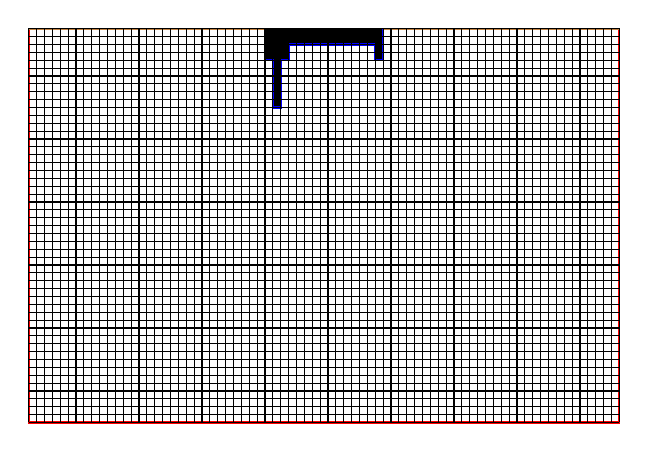
\begin{tikzpicture}
    \draw (0,5.0) -- (0,0) -- (7.5,0) -- (7.5,5.0) -- cycle;
    \draw[fill=black] (3.0,5.0)--(3.0,4.6) -- (3.1,4.6)
      --(3.1,4.0) -- (3.2,4.0) -- (3.2,4.6) --(3.3,4.6) -- (3.3,4.8) -- (4.4,4.8) --
      (4.4,4.6) --
      (4.5,4.6) -- (4.5,5.0) -- cycle; 
    \draw[red, thick] (0,5.0) -- (0,0) -- (7.5,0) -- (7.5,5.0);
    \draw[blue, thick] (3.0,5.0)--(3.0,4.6) -- (3.1,4.6)
      --(3.1,4.0) -- (3.2,4.0) -- (3.2,4.6) --(3.3,4.6) -- (3.3,4.8) -- (4.4,4.8) --
      (4.4,4.6) --
      (4.5,4.6) -- (4.5,5.0); 
    \draw[brown, thick] (0,5.0) -- (3.0,5.0);
    \draw[brown, thick] (4.5,5.0) -- (7.5,5.0);
    \foreach \y in {0,1,...,50}
    \draw[thin] (0, 0.1*\y) -- (7.5,0.1*\y);
    \foreach \x in {0,1,...,75}
    \draw[thin] (0.1*\x,0) -- (0.1*\x, 5.0);

  \end{tikzpicture}
  \caption{二维渗流流函数计算区域}
  \label{fig_2dshenliu_region}
\end{figure}

采用迭代法计算结果如图\ref{FgEx_2dshenliu_flood}和\ref{FgEx_2dshenliu_lines}所示。
不同迭代法的到达收敛所需迭代步数对比见图\ref{FgEx_2dshenliu_iteration}所示。
\begin{figure}[htb]
  \centering
  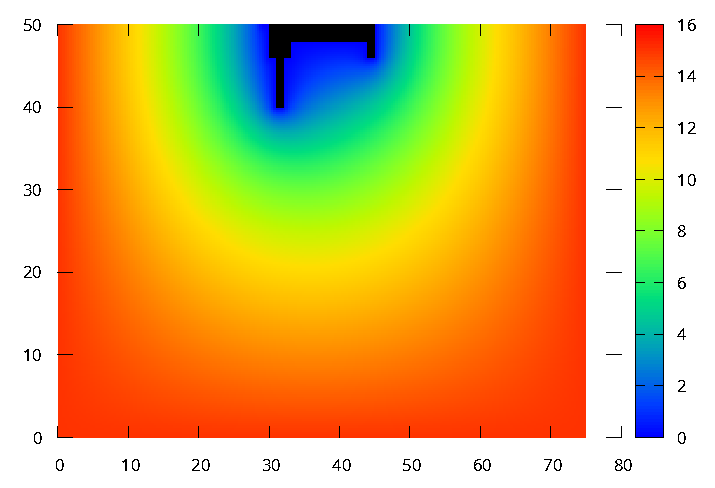
\includegraphics{FgEx_2dshenliu_flood.eps}
  \caption{二维渗流流函数分布云图}
  \label{FgEx_2dshenliu_flood}
\end{figure}
\begin{figure}[htb]
  \centering
  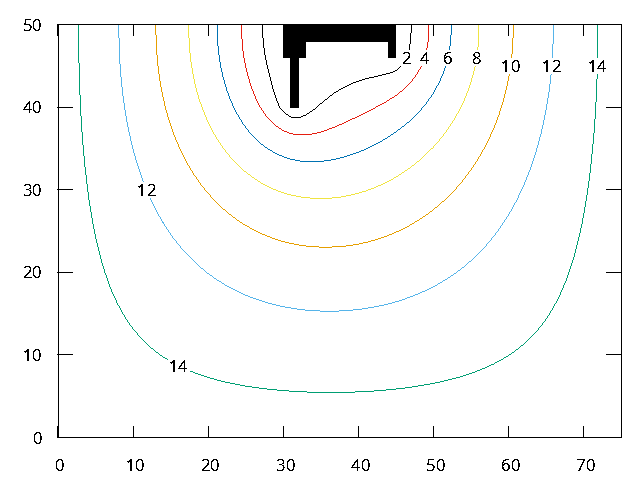
\includegraphics{FgEx_2dshenliu_lines.eps}
  \caption{二维渗流流函数等值线图}
  \label{FgEx_2dshenliu_lines}
\end{figure}
\begin{figure}[htb]
  \centering
  \includegraphics{FgEx_2dshenliu_iteration.pdf}
  \caption{不同迭代法收敛过程对比图}
  \label{FgEx_2dshenliu_iteration}
\end{figure}

%\section{二维方腔顶盖驱动流动求解}
%\subsection{问题描述}
%\subsection{SIMPLE算法求解}
%\subsection{涡量-流函数求解方法}

%\section{二维浅水方程求解}
%\subsection{网格基础}
%\subsection{求解算法}



\end{document}

